\documentclass[journal,12pt,twocolumn]{IEEEtran}

\usepackage{setspace}
\usepackage{gensymb}
\singlespacing
\usepackage[cmex10]{amsmath}

\usepackage{amsthm}

\usepackage{mathrsfs}
\usepackage{txfonts}
\usepackage{stfloats}
\usepackage{bm}
\usepackage{cite}
\usepackage{cases}
\usepackage{subfig}

\usepackage{longtable}
\usepackage{multirow}

\usepackage{enumitem}
\usepackage{mathtools}
\usepackage{steinmetz}
\usepackage{tikz}
\usepackage{circuitikz}
\usepackage{verbatim}
\usepackage{tfrupee}
\usepackage[breaklinks=true]{hyperref}
\usepackage{graphicx}
\usepackage{tkz-euclide}

\usetikzlibrary{calc,math}
\usepackage{listings}
    \usepackage{color}                                            %%
    \usepackage{array}                                            %%
    \usepackage{longtable}                                        %%
    \usepackage{calc}                                             %%
    \usepackage{multirow}                                         %%
    \usepackage{hhline}                                           %%
    \usepackage{ifthen}                                           %%
    \usepackage{lscape}     
\usepackage{multicol}
\usepackage{chngcntr}

\DeclareMathOperator*{\Res}{Res}
\newtheorem{theorem}{Theorem}[section]
\newtheorem{corollary}{Corollary}[theorem]
\newtheorem{lemma}[theorem]{Lemma}
\newtheorem{definition}{Definition}[section]
\renewcommand\thesection{\arabic{section}}
\renewcommand\thesubsection{\thesection.\arabic{subsection}}
\renewcommand\thesubsubsection{\thesubsection.\arabic{subsubsection}}

\renewcommand\thesectiondis{\arabic{section}}
\renewcommand\thesubsectiondis{\thesectiondis.\arabic{subsection}}
\renewcommand\thesubsubsectiondis{\thesubsectiondis.\arabic{subsubsection}}


\hyphenation{op-tical net-works semi-conduc-tor}
\def\inputGnumericTable{}                                 %%

\lstset{
%language=C,
frame=single, 
breaklines=true,
columns=fullflexible
}
\begin{document}

\newcommand{\BEQA}{\begin{eqnarray}}
\newcommand{\EEQA}{\end{eqnarray}}
\newcommand{\define}{\stackrel{\triangle}{=}}
\bibliographystyle{IEEEtran}
\raggedbottom
\setlength{\parindent}{0pt}
\providecommand{\mbf}{\mathbf}
\providecommand{\pr}[1]{\ensuremath{\Pr\left(#1\right)}}
\providecommand{\qfunc}[1]{\ensuremath{Q\left(#1\right)}}
\providecommand{\sbrak}[1]{\ensuremath{{}\left[#1\right]}}
\providecommand{\lsbrak}[1]{\ensuremath{{}\left[#1\right.}}
\providecommand{\rsbrak}[1]{\ensuremath{{}\left.#1\right]}}
\providecommand{\brak}[1]{\ensuremath{\left(#1\right)}}
\providecommand{\lbrak}[1]{\ensuremath{\left(#1\right.}}
\providecommand{\rbrak}[1]{\ensuremath{\left.#1\right)}}
\providecommand{\cbrak}[1]{\ensuremath{\left\{#1\right\}}}
\providecommand{\lcbrak}[1]{\ensuremath{\left\{#1\right.}}
\providecommand{\rcbrak}[1]{\ensuremath{\left.#1\right\}}}
\theoremstyle{remark}
\newtheorem{rem}{Remark}
\newtheorem*{remark}{Remark}
\newcommand{\sgn}{\mathop{\mathrm{sgn}}}
\providecommand{\abs}[1]{\vert#1\vert}
\providecommand{\res}[1]{\Res\displaylimits_{#1}} 
\providecommand{\norm}[1]{\lVert#1\rVert}
%\providecommand{\norm}[1]{\lVert#1\rVert}
\providecommand{\mtx}[1]{\mathbf{#1}}
\providecommand{\mean}[1]{E[ #1 ]}
\providecommand{\fourier}{\overset{\mathcal{F}}{ \rightleftharpoons}}
%\providecommand{\hilbert}{\overset{\mathcal{H}}{ \rightleftharpoons}}
\providecommand{\system}{\overset{\mathcal{H}}{ \longleftrightarrow}}
	%\newcommand{\solution}[2]{\textbf{Solution:}{#1}}
\newcommand{\solution}{\noindent \textbf{Solution: }}
\newcommand{\cosec}{\,\text{cosec}\,}
\providecommand{\dec}[2]{\ensuremath{\overset{#1}{\underset{#2}{\gtrless}}}}
\newcommand{\myvec}[1]{\ensuremath{\begin{pmatrix}#1\end{pmatrix}}}
\newcommand{\mydet}[1]{\ensuremath{\begin{vmatrix}#1\end{vmatrix}}}
\numberwithin{equation}{subsection}
\makeatletter
\@addtoreset{figure}{problem}
\makeatother
\let\StandardTheFigure\thefigure
\let\vec\mathbf
\renewcommand{\thefigure}{\theproblem}
\def\putbox#1#2#3{\makebox[0in][l]{\makebox[#1][l]{}\raisebox{\baselineskip}[0in][0in]{\raisebox{#2}[0in][0in]{#3}}}}
     \def\rightbox#1{\makebox[0in][r]{#1}}
     \def\centbox#1{\makebox[0in]{#1}}
     \def\topbox#1{\raisebox{-\baselineskip}[0in][0in]{#1}}
     \def\midbox#1{\raisebox{-0.5\baselineskip}[0in][0in]{#1}}
\vspace{3cm}
\title{Gate Assignment 2}
\author{Yashas Tadikamalla - AI20BTECH11027}
\maketitle
\newpage
\bigskip
\renewcommand{\thefigure}{\theenumi}
\renewcommand{\thetable}{\theenumi}
Download all python codes from 
\begin{lstlisting}
https://github.com/YashasTadikamalla/EE3900/blob/main/GateAssignment2/codes
\end{lstlisting}
%
and latex-tikz codes from 
%
\begin{lstlisting}
https://github.com/YashasTadikamalla/EE3900/blob/main/GateAssignment2/GateAssignment2.tex
\end{lstlisting}
\section{Problem (EC-2010 Q15)}
Two discrete time systems with impulse responses $h_1[n]=\delta[n-1]$ and $h_2[n]=\delta[n-2]$ are connected in cascade. The overall impulse response of the cascaded system is
\begin{enumerate}
    \item $\delta[n-1]+\delta[n-2]$
    \item $\delta[n-4]$
    \item $\delta[n-3]$
    \item $\delta[n-1]\delta[n-2]$
\end{enumerate}
\section{Solution}
\begin{definition}[Discrete Time Fourier Transform]
It is the member of the Fourier transform family that operates on aperiodic, discrete signals. If $x[n]$ is the input signal in time domain, its DTFT is $X(\Omega)$, a complex function in frequency domain.
\begin{align}
    X(\Omega)=\displaystyle\sum_{k=-\infty}^{\infty}x[k]e^{-j\Omega k} 
\end{align}
\end{definition}
\begin{definition}[Inverse DTFT]
If $X(\Omega)$ is the DTFT of $x[n]$, then $x[n]$ is the inverse DTFT of $X(\Omega)$.
\end{definition}
\begin{lemma}
For any real c, if $x[n]=\delta[n-c]$, then
\begin{align}
    X(\Omega)=e^{-j\Omega c}
    \label{eq:delta}
\end{align}
\end{lemma}
\begin{proof}
\begin{align}
     X(\Omega)&=\displaystyle\sum_{k=-\infty}^{\infty}x[k]e^{-j\Omega k}=\displaystyle\sum_{k=-\infty}^{\infty}\delta[k-c]e^{-j\Omega k}\\
     &=\delta[0]e^{-j\Omega c}=e^{-j\Omega c}
\end{align}
\end{proof}
\begin{corollary}
For any real c, if $X(\Omega)=e^{-j\Omega c}$, then $x[n]=\delta[n-c]$
\end{corollary}
\begin{theorem}[Convolution theorem]If $x[n]=x_1[n]*x_2[n]$, then the DTFT of $x[n]$ can be given by
\begin{align}
    X(\Omega)=X_1(\Omega)X_2(\Omega)\label{eq:con}
\end{align}
\end{theorem}
\begin{theorem}For a cascade system, the overall impulse response is given by
\begin{align}
    h[n]=h_1[n]*h_2[n]\label{eq:oimp}
\end{align}
\end{theorem}
\begin{proof}
Given, two impulse responses $h_1[n],h_2[n]$ in cascade. The output signal $y[n]$ for the input signal $x[n]$ is given by
\begin{align}
    y[n]&=h_2[n]*\brak{h_1[n]*x}\\
    &=\brak{h_2[n]*h_1[n]}*x[n]\\
    &=\brak{h_1[n]*h_2[n]}*x[n]\\
    &=h[n]*x[n]
\end{align}
$h[n]=h_1[n]*h_2[n]$ is overall impulse response. (Convolution is associative and commutative)
\end{proof}
Given,
\begin{align}
    h_1[n]=\delta[n-1]\\
    h_2[n]=\delta[n-2]
\end{align}
To find: $h(t)$. We know, 
\begin{align}
h[n]=h_1[n]*h_2[n]
\end{align}
From \eqref{eq:con}
\begin{align}
H(\Omega)=H_1(\Omega)H_2(\Omega)
\end{align}
Using \eqref{eq:delta}, 
\begin{align}
H(\Omega)&=e^{-j\Omega}e^{-2j\Omega}=e^{-3j\Omega}\\
\Rightarrow h[n]&=\delta[n-3]
\end{align}
Option 3 is the correct answer.
\begin{theorem}
If $y[n]=x[n]*\delta[n-n_0]$, then $y[n]=x[n-n_0]$
\end{theorem}
\begin{proof}
\begin{align}
    y[n]&=x[n]*\delta[n-n_0]\\
    &=\displaystyle\sum_{k=-\infty}^{\infty} x[k]\delta[n-n_0-k]\\
    &=x[n-n_0]
\end{align}
\end{proof}
\begin{figure}[!h]
 \centering
 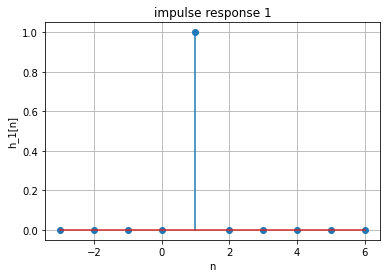
\includegraphics[width=\columnwidth]{GateAssignment2(1).png}
 \caption{Plot of $h_1[n]=\delta[n-1]$}
 \label{plot}
\end{figure}
\begin{figure}[!h]
 \centering
 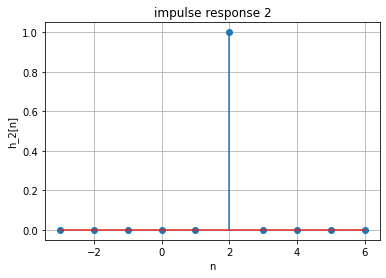
\includegraphics[width=\columnwidth]{GateAssignment2(2).png}
 \caption{Plot of $h_2[n]=\delta[n-2]$}
 \label{plot}
\end{figure}
\begin{figure}[!h]
 \centering
 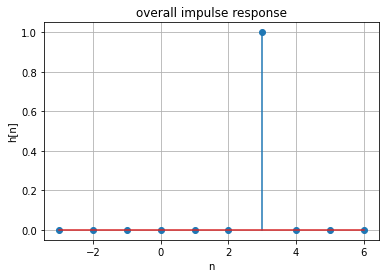
\includegraphics[width=\columnwidth]{GateAssignment2(3).png}
 \caption{Plot of $h[n]=\delta[n-3]$}
 \label{plot}
\end{figure}
\end{document}


